% Chapter where we present the results.

\chapter{Results}
\label{ch:results}

In Chapter \ref{ch:methods} we discussed a general solution to the protoboard
layout problem, and various alternatives that can be used in implementing the
solution. Figure \ref{fig:alternatives} presents the alternatives in a structured
way. Here, we will explore these alternatives and compare them quantitatively.
This section will provide data that is useful in comparing the alternatives, and
the data will be discussed in detail in Chapter \ref{ch:discussion}.

\begin{figure}[H]
\Tree [.{All Alternatives}
    [{Distance} {Block} ].Placement !\qsetw{4cm}
    [{AP}
     [I D ].{PN}
     [I D ].{PP} ].Wiring !\qsetw{4cm}
    [{Component} {Wire} ].Resistors !\qsetw{4cm}
    [$A*$ {Best First} ].Search ]
\label{fig:alternatives}
\caption{All possible alternatives to the algorithm.}
\end{figure}

The data to compare the alternatives is gathered as described in Chapter
\ref{ch:methods}. We run the algorithm on $4425$ randomly generated schematics
of varying complexities. The algorithm is run $10$ times on each schematic.

In comparing alternatives, there are $3$ items we will consider:
\begin{enumerate}
\item Which alternative is the most successful?
\item Which alternative, when successful, takes the least amount of time?
\item Which alternative, when successful, produces the best layouts?
\end{enumerate}

In comparing success time, we will look at CPU time spent on the wiring step, as
the placement step has much less variability. We will look at plots of circuit
complexity versus wiring times to do the comparisons. Our measure of complexity
of a circuit will be the number of pins in the circuit as discussed in Chapter
\ref{ch:methods} (TODO: this is currently not done, be sure to give a histogram
of numbers of pins in the circuits).

In comparing the goodness of layouts, we will compare numbers of wires, total
lengths of wires, and numbers of wire crosses.

\section{Comparing placement methods}
\label{sec:compare_placement}

We have two placement methods available: choosing a placement that aims to
minimize the sum of pairwise distances between pairs of points on the protoboard
that need to be interconnected, and choosing a placement that aims to minimize
the number of rows blocked off (in some sense) in each column. To compare these
two placement methods, we keep the other alternatives fixed at some choices.
In the data given below, the wiring method used is per-pair wiring, in decreasing
order of distances apart, resistors are treated as components, and we use $A*$ as
our search algorithm.

First we look at the success rates that result from the two placement methods.
Figure \ref{fig:placement_success} presents a bar graph that compares the numbers
of times, out of $10$ runs, each method succeeded over the $4425$ schematics.
Table \ref{tb:placement_success} presents the same data more precisely.

\begin{figure}[H]
\begin{center}
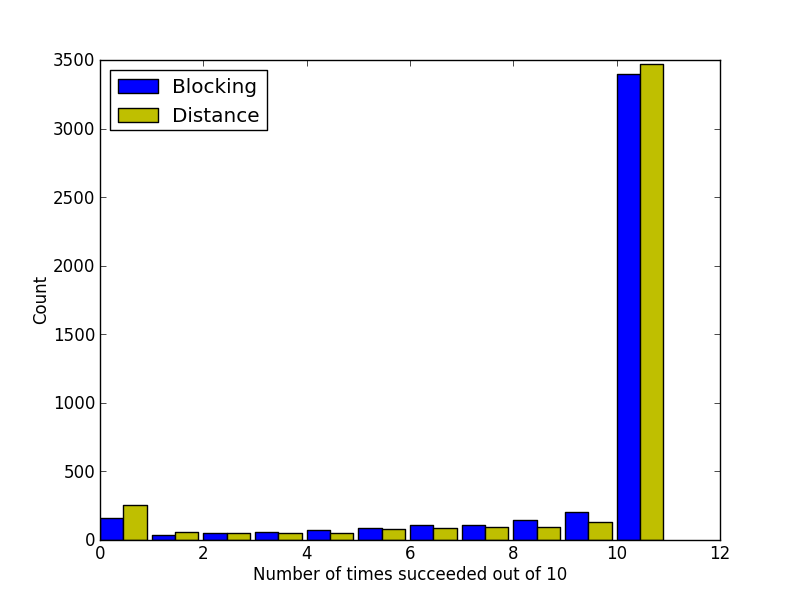
\includegraphics[width=\textwidth]{Images/placement_success_comparison.png}
\caption{Placement method comparison: success rates.}
\label{fig:placement_success}
\end{center}
\end{figure}

\begin{table}[H]
\begin{center}
\begin{singlespace}
\begin{tabular}{|c||c|c|c|c|c|c|c|c|c|c|c|}
\hline
 & \multicolumn{11}{|c|}{Number of times succeeded out of $10$} \\
\hline
 & 0 & 1 & 2 & 3 & 4 & 5 & 6 & 7 & 8 & 9 & 10 \\
\hline\hline
Blocking & $162$ & $38$ & $51$ & $57$ & $72$ & $85$ & $109$ & $106$ & $144$ & $203$ & $3398$ \\
 & $0.04$ & $0.01$ & $0.01$ & $0.01$ & $0.02$ & $0.02$ & $0.02$ & $0.02$ & $0.03$ & $0.05$ & $0.77$ \\
\hline
 Distance & $258$ & $55$ & $54$ & $50$ & $52$ & $77$ & $86$ & $97$ & $93$ & $130$ & $3473$ \\
  & $0.06$ & $0.01$ & $0.01$ & $0.01$ & $0.01$ & $0.02$ & $0.02$ & $0.02$ & $0.02$ & $0.03$ & $0.78$ \\
\hline
\end{tabular}
\end{singlespace}
\end{center}
\label{tb:placement_success}
\caption{Placement method comparison: success rates.}
\end{table}

Next we look at the trends of success for the two methods as circuits get more
complex. Figure \ref{fig:placement_success_trend} presents the average success
rate at each discrete complexity level.

\begin{figure}[H]
\begin{center}
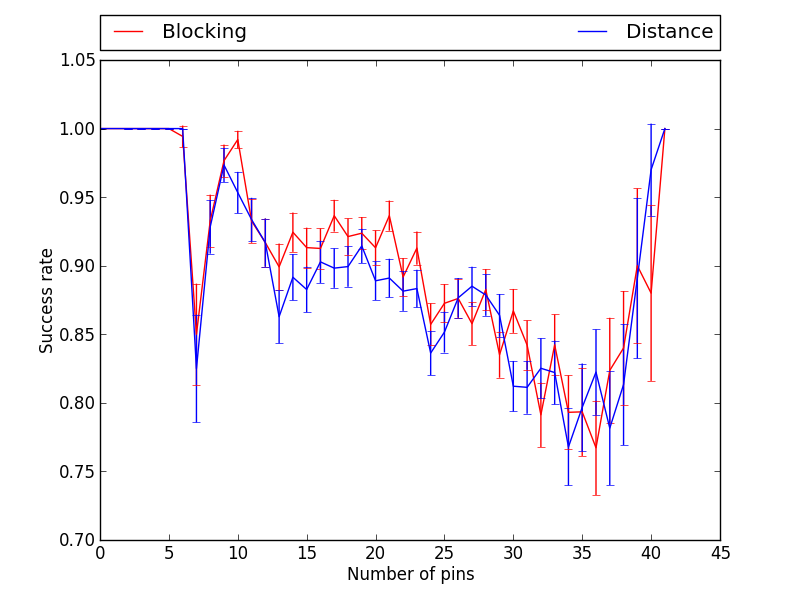
\includegraphics[width=\textwidth]{Images/placement_success_trend_comparison.png}
\caption{Placement method comparison: success rate trends.}
\label{fig:placement_success_trend}
\end{center}
\end{figure}

Now we look at the trends of wiring time for the two methods as circuits get
more complex. Figure \ref{fig:placement_time_trend} presents the average wiring
time (in seconds) at each discrete complexity level.

\begin{figure}[H]
\begin{center}
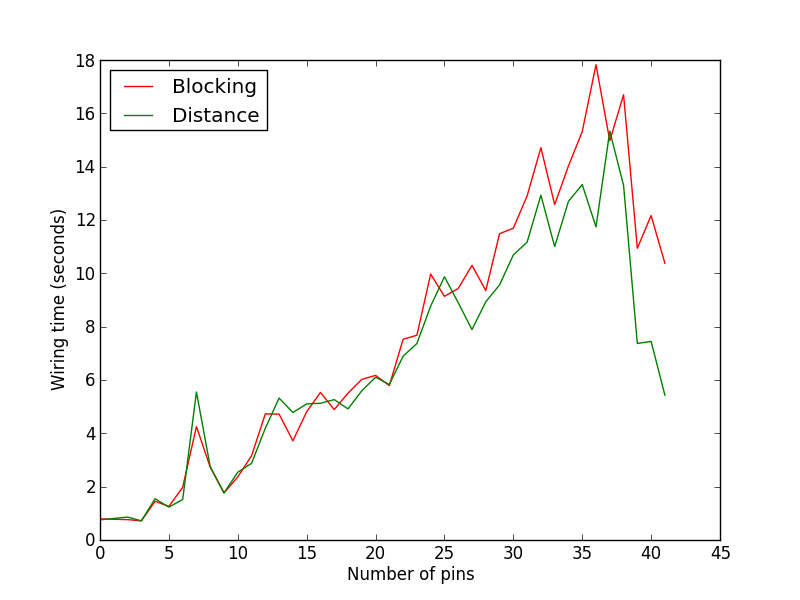
\includegraphics[width=\textwidth]{Images/placement_time_trend_comparison.png}
\caption{Placement method comparison: wiring time trends.}
\label{fig:placement_time_trend}
\end{center}
\end{figure}

Finally wee look at the quality of the layouts the two alternative placement
methods produces. Figure \ref{fig:placement_quality_trend} gives average number of
wires, average number of wire crosses, and average total lengths of wires at
each discrete complexity level.

\begin{figure}
\begin{center}
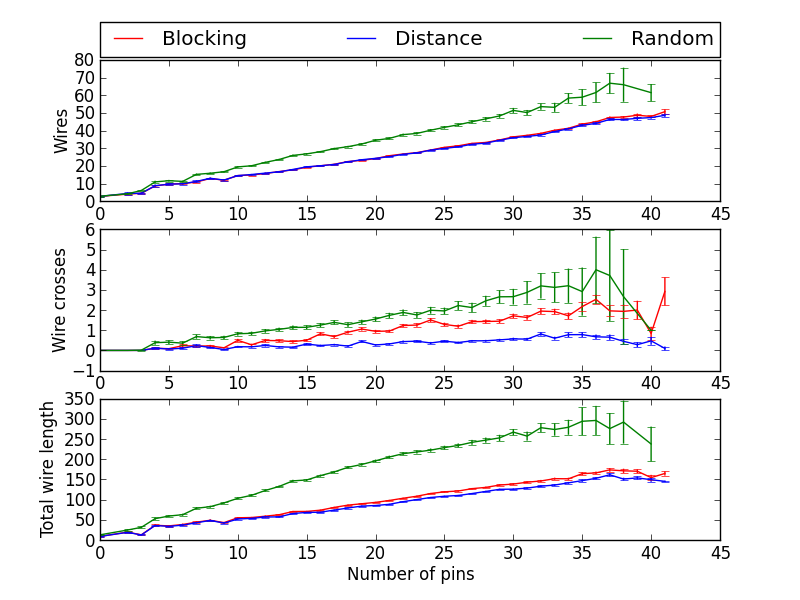
\includegraphics[width=\textwidth]{Images/placement_quality_trend_comparison.png}
\caption{Placement method comparison: layout quality trends.}
\label{fig:placement_quality_trend}
\end{center}
\end{figure}

Discussion of all of these results follows in Chapter \ref{ch:discussion}.

\section{Comparing wiring methods}

\section{Comparing resistor treatments}

\section{Comparing search methods}

\section{Putting them all together}

\section{Exemplars}
